\pgfplotsset{
    colormap={custom_blue}{
        rgb255(0cm)=(255,255,255);
        rgb255(1cm)=(0,0,255)
    }
}

\begin{figure}[t]
    \centering
    \begin{minipage}{0.78\textwidth}
        \centering

        % \tikzstyle{rectanglenode}=[rectangle, inner sep=0,fill=blue!70];
        
        \subfloat[DPO]{
            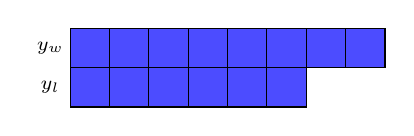
\begin{tikzpicture}[scale=0.5]
                % \node [anchor=north, font=\tiny, align=center]
                % (eq01) at (0,0) {$\beta r(y^w,\pi_{ref})-\beta r(y^l,\pi_{ref})$}
                \foreach \i in {1,...,8} {
                    \draw[fill=blue!70] (\i, 1) rectangle (\i+1, 2);
                }
                \foreach \i in {1,...,6} {
                    \draw[fill=blue!70] (\i, 0) rectangle (\i+1, 1);
                }
                \node at (0.5, 1.5) {\scriptsize $y_w$};
                \node at (0.5, 0.5) {\scriptsize $y_l$};
                % \node at (0.0, 2.5) {\scriptsize $\beta r(y^w,\pi_{ref})-\beta r(y^l,\pi_{ref})$};
            \end{tikzpicture}
        }
        \hspace{0.15in}
        \subfloat[SimPO]{
            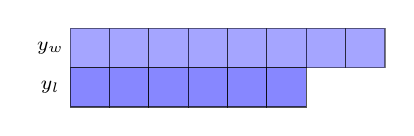
\begin{tikzpicture}[scale=0.5]
                \foreach \i in {1,...,8} {
                    \draw[fill=blue!70,opacity=0.5] (\i, 1) rectangle (\i+1, 2);
                }
                \foreach \i in {1,..., 6} {
                    \draw[fill=blue!70,opacity=0.67] (\i, 0) rectangle (\i+1, 1);
                }
                \node at (0.5, 1.5) {\scriptsize $y_w$};
                \node at (0.5, 0.5) {\scriptsize $y_l$};
                % \node at (0.0, 2.5) {\scriptsize $\beta r(y^w,\pi_{ref})-\beta r(y^l,\pi_{ref})$};
            \end{tikzpicture}
        }
        \hspace{0.15in}
        \subfloat[SamPO]{
            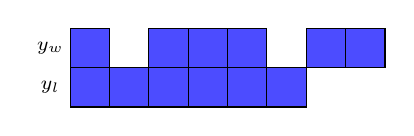
\begin{tikzpicture}[scale=0.5]
                \foreach \i in {1,3,4,5,7,8} {
                    \draw[fill=blue!70] (\i, 1) rectangle (\i+1, 2);
                }
                \foreach \i in {1,...,6} {
                    \draw[fill=blue!70] (\i, 0) rectangle (\i+1, 1);
                }
                \foreach \i in {2, 6} {
                    \draw[fill=blue!70,opacity=0] (\i, 1) rectangle (\i+1, 2);
                }
                \node at (0.5, 1.5) {\scriptsize $y_w$};
                \node at (0.5, 0.5) {\scriptsize $y_l$};
            \end{tikzpicture}
        }
        \hspace{0.15in}
        \subfloat[\method (Ours)]{
            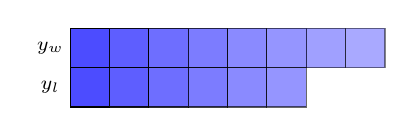
\begin{tikzpicture}[scale=0.5]
                \foreach \i in {1,...,8} {
                    \pgfmathsetmacro{\opacity}{0.9^(\i - 1)};
                    \draw[fill=blue!70,opacity=\opacity] (\i, 1) rectangle (\i+1, 2);
                }
                \foreach \i in {1,...,6} {
                    \pgfmathsetmacro{\opacity}{0.9^(\i - 1)};
                    \draw[fill=blue!70,opacity=\opacity] (\i, 0) rectangle (\i+1, 1);
                }
                \node at (0.5, 1.5) {\scriptsize $y_w$};
                \node at (0.5, 0.5) {\scriptsize $y_l$};
            \end{tikzpicture}
        }
    \end{minipage}
    \begin{minipage}{0.1\textwidth}
        \centering
        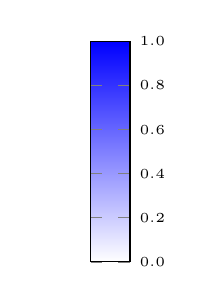
\begin{tikzpicture}
            \begin{axis}[
                hide axis,
                scale only axis,
                height=2.8cm,
                width=0.6cm,
                colorbar,
                colormap name=custom_blue, % 你可以选择其他的色彩图,例如 'hot', 'cool', 'jet', 'parula' 等
                point meta min=0,
                point meta max=1,
                colorbar style={
                    ytick={0, 0.2, 0.4,..., 1.0},
                    % ylabel={\scriptsize Weight},
                    yticklabel style={font=\tiny,
                    /pgf/number format/fixed,/pgf/number format/fixed zerofill,/pgf/number format/precision=1},
                },
            ]
            \addplot [draw=none] coordinates {(0,0) (1,1)};
            \end{axis}
        \end{tikzpicture}
        
    \end{minipage}

    \caption{Illustration of coefficients in DPO, SimPO, SamPO, and our \method across various positions. Each box represents a coefficient, and the opacity denotes the magnitude, with darker colors indicating higher values. (a) For DPO, the coefficients are uniform across different positions. (b) For SimPO, the coefficients of the chosen $y_w$ and the rejected $y_l$ are normlaized by their lengths $|y_w|$ and $|y_l|$, respectively. (c) In SamPO, the coefficients are selected based on the minimum length of $|y_w|$ and $|y_l|$. (d) Our method introduces a $\gamma$ factor to implement coefficient decay, specifically as a sequence defined by $\gamma^t$ (e.g., 1, $\gamma$, $\gamma^2$, ..., $\gamma^T$). Here, we use $\gamma=0.9$ for a clear visualization.}
    \label{fig:decay_mechanisms}
\end{figure}



% \newlength{\seg}
%     \setlength{\seg}{2.0em}
%     \newlength{\subseg}
%     \setlength{\subseg}{8em}
%     \newlength{\resseg}
%     \setlength{\resseg}{1.3em}

% \begin{figure}[t]
%     \centering
%     \begin{minipage}{0.78\textwidth}
%         \centering

%         \tikzstyle{rectanglenode}=[rectangle,minimum height=1.5em,minimum width=1.5em, inner sep=0,fill=blue!70, draw=black, line width=0pt];
        
%         \subfloat[DPO]{
%             \begin{tikzpicture}[scale=0.5]
%                 \node [anchor=north, font=\tiny, align=center]
%                 (eq01) at (0,0) {$\beta r(y^w,\pi_{ref})-\beta r(y^l,\pi_{ref})$ };

                
%                 \foreach \i in {1,...,8} {
%                     \node[rectanglenode] at (\i+0.5, 1.5) {};
%                 }
%                 \foreach \i in {1,...,6} {
%                     \node[rectanglenode] at (\i+0.5, 0.5) {};
%                 }
%                 \node at (0.5, 1.5) {\scriptsize $y_w$};
%                 \node at (0.5, 0.5) {\scriptsize $y_l$};
%             \end{tikzpicture}
%         }
        % \hspace{0.15in}
        % \subfloat[SimPO]{
        %     \begin{tikzpicture}[scale=0.5]
        %         \foreach \i in {1,...,8} {
        %             \draw[fill=blue!70,opacity=0.5] (\i, 1) rectangle (\i+1, 2);
        %         }
        %         \foreach \i in {1,..., 6} {
        %             \draw[fill=blue!70,opacity=0.67] (\i, 0) rectangle (\i+1, 1);
        %         }
        %         \node at (0.5, 1.5) {\scriptsize $y_w$};
        %         \node at (0.5, 0.5) {\scriptsize $y_l$};
        %         % \node at (0.0, 2.5) {\scriptsize $\beta r(y^w,\pi_{ref})-\beta r(y^l,\pi_{ref})$};
        %     \end{tikzpicture}
        % }
        % \hspace{0.15in}
        % \subfloat[SamPO]{
        %     \begin{tikzpicture}[scale=0.5]
        %         \foreach \i in {1,3,4,5,7,8} {
        %             \draw[fill=blue!70] (\i, 1) rectangle (\i+1, 2);
        %         }
        %         \foreach \i in {1,...,6} {
        %             \draw[fill=blue!70] (\i, 0) rectangle (\i+1, 1);
        %         }
        %         \foreach \i in {2, 6} {
        %             \draw[fill=blue!70,opacity=0] (\i, 1) rectangle (\i+1, 2);
        %         }
        %         \node at (0.5, 1.5) {\scriptsize $y_w$};
        %         \node at (0.5, 0.5) {\scriptsize $y_l$};
        %     \end{tikzpicture}
        % }
        % \hspace{0.15in}
        % \subfloat[Ours]{
        %     \begin{tikzpicture}[scale=0.5]
        %         \foreach \i in {1,...,8} {
        %             \pgfmathsetmacro{\opacity}{0.9^(\i - 1)};
        %             \draw[fill=blue!70,opacity=\opacity] (\i, 1) rectangle (\i+1, 2);
        %         }
        %         \foreach \i in {1,...,6} {
        %             \pgfmathsetmacro{\opacity}{0.9^(\i - 1)};
        %             \draw[fill=blue!70,opacity=\opacity] (\i, 0) rectangle (\i+1, 1);
        %         }
        %         \node at (0.5, 1.5) {\scriptsize $y_w$};
        %         \node at (0.5, 0.5) {\scriptsize $y_l$};
        %     \end{tikzpicture}
        % }
%     \end{minipage}
%     \begin{minipage}{0.1\textwidth}
%         \centering
%         \begin{tikzpicture}
%             \begin{axis}[
%                 hide axis,
%                 scale only axis,
%                 height=2.8cm,
%                 width=0.6cm,
%                 colorbar,
%                 colormap name=custom_blue, % 你可以选择其他的色彩图,例如 'hot', 'cool', 'jet', 'parula' 等
%                 point meta min=0,
%                 point meta max=1,
%                 colorbar style={
%                     ytick={0, 0.2, 0.4,..., 1.0},
%                     % ylabel={\scriptsize Weight},
%                     yticklabel style={font=\tiny,
%                     /pgf/number format/fixed,/pgf/number format/fixed zerofill,/pgf/number format/precision=1},
%                 },
%             ]
%             \addplot [draw=none] coordinates {(0,0) (1,1)};
%             \end{axis}
%         \end{tikzpicture}
%     \end{minipage}

%     \caption{Illustration of coefficients in DPO, SimPO, SamPO, and our method, across various positions. Each box represents a coefficient, and the opacity denotes the dark color denotes a higher. (a) For DPO, the coefficients are uniform across different positions. (b) For SimPO, the coefficients of the chosen $y_w$ and the rejected $y_l$ are normlaized by its length $|y_w|$ and $|y_l|$, respectively. (c) In SamPO, the coefficients are selected based on the minimum length of $|y_w|$ and $|y_l|$. (d) Our method introduces a $\gamma$ factor controlling the coefficients, which decay according to $\gamma^t$ (e.g., 1, $\gamma$, $\gamma^2$, ..., $\gamma^T$).}
%     \label{fig:decay_mechanisms}
% \end{figure}





